\RequirePackage[T1]{fontenc}
\documentclass[conference]{IEEEtran}
\usepackage{amsmath,amssymb}
\usepackage{newtxtext,newtxmath}
\usepackage{graphicx}
\graphicspath{{paper/figures/}{figures/}}
\usepackage{booktabs}
\usepackage{balance}
\usepackage{url}
\usepackage[hidelinks]{hyperref}
\title{Consequa-X: An Evidence and Intervention Protocol for Consequential Agent Actions}
\author{\IEEEauthorblockN{Devrajsinh Jhala}}
\begin{document}
\raggedbottom
\maketitle

\begin{abstract}
A lost acknowledgement can turn a successful agent action into a duplicate
when the agent retries. Reliable diagnosis must distinguish what the agent
reported, whether the requested state holds and which actor produced it.
Consequa-X contributes an evidence protocol that preserves those distinctions,
observation-specific provenance and explicit unknown verdicts. Its optional
research adapter adds a declared on-reach intervention game and refusal-aware
accounting around existing contrastive and permutation Shapley estimators.
Across 2,048 scripted-simulator sampling trials, all 655,360 planned replay
branches were retained, including invalid and unstarted branches. At one
predeclared retry coefficient, nominal normal intervals covered the reference
in 118/128 trials; Hoeffding bounds covered in 128/128 but detected its sign in
only 8/128. A separate 24-episode, single-model exploratory validation found
six contradicted status claims among ten assessable claims for one prompt.
These results support testable protocol properties and expose the availability
and precision costs of the declared evidence and replay rules. Comparative
accuracy, real-service effectiveness and broad model generalization remain open.
\end{abstract}

\begin{IEEEkeywords}
agent systems, outcome verification, evidence provenance, counterfactual replay,
software artifacts, uncertainty
\end{IEEEkeywords}

\section{Introduction}
A consequential tool operation has distinct stages: selection, dispatch,
execution, response, reported assessment and external observation. A service
can commit an effect before its acknowledgement is lost. Retrying can create
another effect unless the logical operation's identity and idempotency semantics
are retained. Conversely, a successful response can coexist with an incomplete
or incorrect effect. Explaining such runs requires more than reading the last
tool response or the agent's prose.

State satisfaction and effect origin also differ. An external refund may
satisfy the requested balance or count while remaining unlinked to this agent.
A source-supported origin link is a provenance claim; it does not establish
counterfactual necessity. A replay effect is a separate claim about a declared
intervention, continuation policy and outcome distribution.

Consequa-X makes these distinctions inspectable. Its core contains typed
records, schema validation, application verification and evidence-only
explanation. Its research adapters provide isolated refund worlds, public-only
policy inputs, a local Ollama adapter and bounded replay experiments. Reported
assessments are captured outputs, not measurements of hidden reasoning.

The paper centers three testable protocol claims:
\begin{enumerate}
\item \textbf{C1: State and origin remain separate.} A satisfied contract can
retain an other-actor or unknown origin. Successive readbacks retain their own
supporting witnesses rather than transferring provenance between observations.
Verification and graph tests exercise external-actor, missing-provenance and
conflicting-witness cases; the local validation contains an other-actor example.
\item \textbf{C2: The replay game is explicit.} On-reach semantics define how
normal early termination treats later requested holds. Strict and on-reach
results remain separate. Analytic enumeration and the variable-length controls
test this distinction; Appendix~\ref{app:games} states its formal scope.
\item \textbf{C3: Refusal remains observable.} Every planned branch is retained
with call accounting; incomplete evidence or an invalid draw refuses affected
estimates. The repeated-sampling study accounts for all 655,360 slots and
reports availability beside numerical accuracy.
\end{enumerate}
These are implementation and declared-game claims. The contribution combines
them in a portable protocol around existing estimators; an equally informed
baseline comparison has not yet established their empirical advantage.
Figure~\ref{fig:architecture} separates the captured-evidence core from the
explicitly invoked research replay path.

\begin{figure*}[t]
\centering
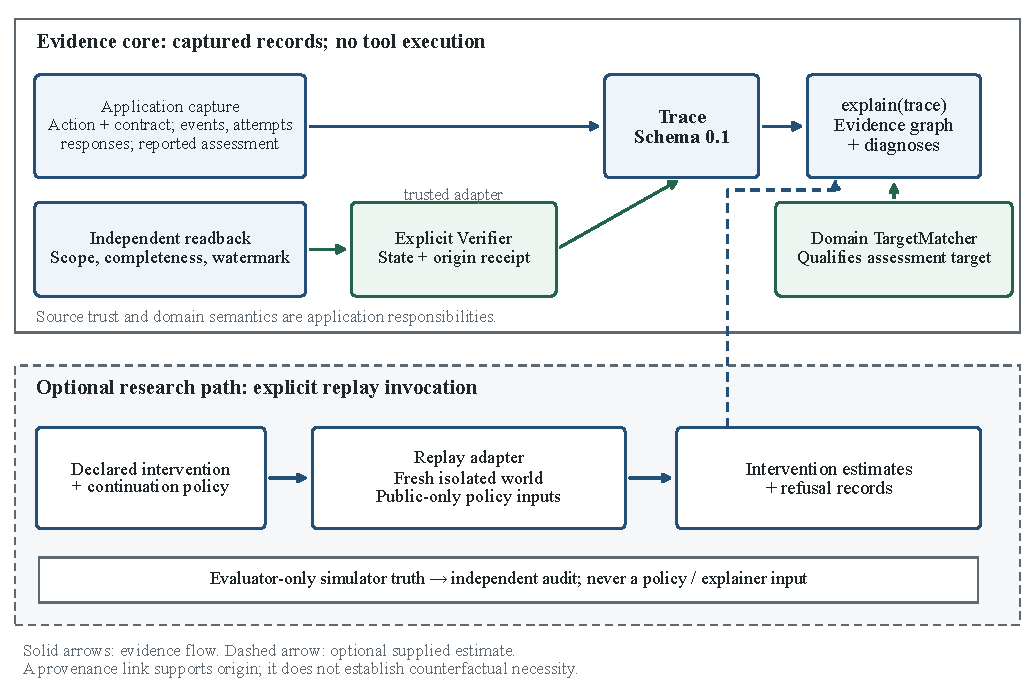
\includegraphics[width=\textwidth]{diagram-evidence-architecture.pdf}
\caption{Evidence flow and trust boundaries. Application verifiers interpret
independent readback; explanations use captured evidence. Explicitly invoked
replay can supply estimates, while evaluator truth remains audit-only. Source
trust and domain semantics remain application responsibilities.}
\label{fig:architecture}
\end{figure*}

\section{Related Work}
Causal Agent Replay (CAR) performs same-policy interventions on recorded
decisions, evaluates user-specified outcomes and uses contrastive suffix and
permutation Shapley attribution~\cite{car}. Consequa-X implements an independent
binary adaptation with its own typed-world, evidence and refusal boundaries.
Applying a verified outcome to replay is therefore not an estimator novelty
claim. Policy-Conditioned Counterfactual Credit studies changes in final
verified success under specified interventions and a continuation
policy~\cite{pccc}; its learning objective differs from post-hoc external-effect
diagnosis, but verified targets and valid interventions are shared concerns.

CausalLoss-Fin jointly intervenes on agent decisions and repairable
infrastructure messages~\cite{causalloss}. Its deterministic programmatic
evaluation limits transfer to stochastic language policies, but it already
occupies the broad combination of financial effects and joint decision/fault
attribution. A future comparison must expose applicable variables to every
method rather than charge omitted infrastructure effects to decisions.

Verified Tool Calls distinguishes acknowledgements from independently checked
effects and uses unknown postcondition conclusions~\cite{verified}.
Callability Is Not Operability studies controlled interface ambiguity and
terminal agent claims~\cite{operability}. Three-valued verification and
response/effect separation are foundations and comparison requirements here.
These targeted primary-source checks do not constitute a systematic review or
an independent reproduction of those papers' empirical results.

Who\&When attributes failed multi-agent runs to an agent and decisive step
from annotated logs~\cite{whoandwhen}; this differs from verifying a particular
external effect from an independent witness. PROV-DM already represents entities,
activities, agents and responsibility~\cite{prov}. Consequa-X is neither a new
general provenance model nor a PROV conformance implementation. Its narrower
contribution is an executable protocol linking temporal contracts, observation
witnesses, separate origin verdicts and explicit refusal.

Agent--tool anomaly work already separates external events from runtime
observations, including exogenous effects~\cite{agenttool}; LIMBO grades
committed-effect histories and analyzes late commits~\cite{limbo}. Response/effect
separation and effect ledgers are therefore prior concepts. Our study audits
a particular protocol rather than establishing a safer recovery controller.
LIMBO's late-commit argument assumes a keyless, non-idempotent write with no
known finite in-flight bound and finite task-completion time. Under those
conditions, bounded watermark polling cannot guarantee exactly-once execution.
Idempotence and eventual consistency are established systems concerns~\cite{helland,vogels}.

AppWorld, ToolSandbox and $\tau$-bench already evaluate world-state outcomes
or stateful trajectories~\cite{appworld,toolsandbox,taubench}. They provide
future transfer targets; this paper evaluates none of their task populations.
For statistics, known binomial Wald-interval limitations~\cite{brown} motivate
careful interval checks but do not by themselves establish paired-Shapley
undercoverage. Modern bounded-mean betting intervals~\cite{betting} are planned
comparators, with the sampling unit and stopping rule still requiring explicit
validation for this replay setting.

\section{Evidence Protocol and Core Interfaces}
\subsection{Objects, contracts and trust}
Let $H$ be visible history, $A$ a logical action, $E$ an execution attempt,
$R$ its response, $B$ a timestamped reported assessment and $O$ an independent
readback observation. A contract $C$ declares payload, count, deadline and
stability horizon. The verifier conclusion $V(C,O)$ is satisfied, violated or
unknown. Origin is separately confirmed, other actor or unknown. Evaluator-only
simulator truth never becomes a policy or explainer input.

The built-in refund predicate uses integer currency minor units. An eligible
effect matches payment, amount and currency, commits in the declared time
window and persists through the horizon. Exact-count contracts also constrain
the count during the stability interval. A stale watermark or inadequate scope
and completeness yields unknown rather than a confident absence claim.
Source authority, scope, completeness and watermark declarations remain trusted
adapter inputs. Schemas and hashes validate structure and changed bytes, not
source authenticity or real transactional guarantees.
Figure~\ref{fig:timeout} illustrates why a response and a reported assessment
cannot substitute for a horizon-covering outcome observation.

\begin{figure*}[t]
\centering
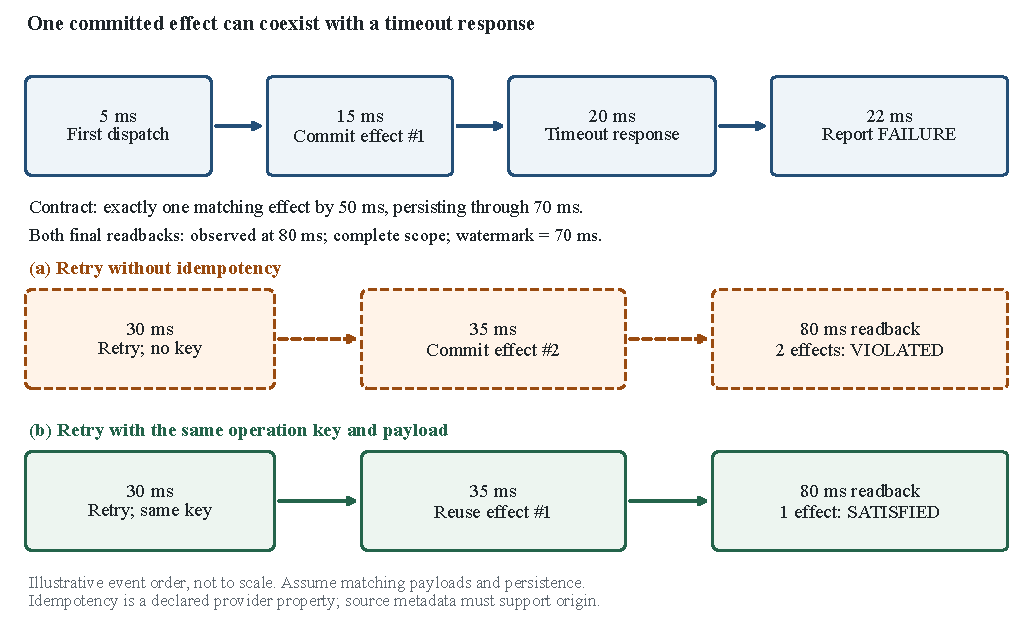
\includegraphics[width=\textwidth]{diagram-timeout-retry.pdf}
\caption{Illustrative timeout-after-commit sequence. A committed effect precedes
a timeout and reported failure. An unsafe retry creates a duplicate; reusing the
same provider-scoped idempotency key and payload preserves one effect. Complete
final readback covers the stability horizon. Arrows show event order, and times
are illustrative rather than sampled observations.}
\label{fig:timeout}
\end{figure*}

\subsection{Reusable application boundary}
The evidence core can operate on a production application's captured records
without any replay. A read-only adapter obtains independent observations;
verification returns state and origin conclusions, and explanation renders the
supporting evidence. This path requires neither simulator reset nor a second
execution of a consequential action.

Applications can supply an explicit read-only verifier through
\texttt{verify(action, observation, verifier=...)}. The wrapper checks receipt
type, contract identity, observation identity, source, watermark and timing.
Domain predicate semantics, authentication and read-only adapter behavior are
the application's responsibility. There is no evaluation of arbitrary predicate
strings. An offline artifact-delivery example constructs captured records and
checks independently read-back content digests without importing the refund
simulator or executing writes.

\texttt{explain(trace)} reads a captured verification and performs no replay.
Refund target matching is built in; other predicates receive a neutral
explanation unless a trusted domain matcher explicitly qualifies attributable
effects against payload and temporal rules. Matchers can return only unique
IDs within the receipt's attributable IDs. Unknown receipts are not interpreted
as target matches. A qualified provenance link still is not a causal effect.

\subsection{Successive witnesses and graph meanings}
Repeated readbacks can disagree about the same effect identifier. The graph
therefore retains observation-specific witnesses and an identity-only shared
effect node. Dispatch-to-effect edges attach to the witness supplying origin
metadata; verification edges use witnesses in that receipt's own observations.
A later conflicting actor, corrected payload or reversal cannot overwrite an
earlier witness and inherit its unqualified origin link. Shared identifiers do
not authenticate or reconcile the records. Estimated-influence edges require
captured event identifiers and an explicitly supplied intervention estimate.

\section{Replay Targets, Games and Uncertainty}
\subsection{Targets and conditional suffix effects}
The refund adapter exposes three targets: initial action selection, global
state-contract satisfaction and action-linked consequence. A known global
violation is false for the linked target. Satisfied state with exclusively
external qualifying effects is false for that target; insufficient provenance
can instead yield unknown. The linked target combines global satisfaction and
qualifying operation-linked witnesses rather than reconstructing an agent-only
world. Unknown observations do not acquire numeric labels.

For known binary target $Z$, set bad outcome $X=1-Z$. Prefix replay holds
factual decisions before position $k$ and resamples the suffix. With one
observed factual bad label $x_f$, the conditional estimand is
\begin{equation}
\gamma_k = \mathbb{E}[X\mid \text{prefix held, suffix resampled at }k]-x_f.
\end{equation}
The factual term is one observed constant, not a population rate estimate.
This factual-anchored target answers: how often would a fresh suffix avoid the
bad outcome observed in this episode? It is useful for episode diagnosis, but
does not estimate the effect of changing one decision against an independently
resampled original arm. That population contrast would instead compare two
expectations, for example $\mathbb{E}[X\mid\text{hold }k]-
\mathbb{E}[X\mid\text{resample }k]$, with the other conditions declared.
Neither estimand is generally preferable; they answer different questions and
have different sampling costs. Here negative $\gamma_k$ indicates rescue
relative to the observed episode. An earlier irrelevant position can have a
nonzero suffix effect because its suffix contains a later stochastic choice.
The \emph{pivot} is the latest position with negative population suffix effect
under this definition. The retained nominal selector attempts to detect that
position only if all planned positions are estimable. Its pointwise intervals
give no simultaneous or post-selection coverage guarantee; selected pivots are
exploratory diagnostics rather than unique causes.

\subsection{Held-decision coalition games}
Let $N$ be reached factual positions. Coalition $S$ requests holding captured
decisions at positions in $S$; other decisions are sampled. Reached held
decisions must match the typed public stage. In the \emph{strict} game, an
earlier termination leaving a requested held position unreachable invalidates
the draw. Finite samples avoiding invalidity do not define the population game.

The separate \emph{on-reach} game treats requested positions beyond a normal
termination as inactive and uses the actual completed episode. Reached
incompatible operations remain invalid; provider failures and exhausted budgets
are not normal inactivity. This is an explicit alternative game, not a repair
of retained strict results.

For a defined game $v(S)=\mathbb{E}[X\mid S]$, signed Shapley values allocate
the held-decision effect~\cite{shapley}:
\begin{equation}
\phi_i = \sum_{S\subseteq N\setminus\{i\}}
\frac{|S|!(|N|-|S|-1)!}{|N|!}\,[v(S\cup\{i\})-v(S)].
\end{equation}
Fresh forward/reverse permutation walks form one paired contribution vector.
Independent empty/full draws diagnose the endpoint scale. Values are signed
allocations under the declared game, not normalized responsibility shares.
Positive values mean holding the factual decision increases bad outcomes;
negative values mean it is protective.

\subsection{Intervals and refusals}
Contrastive defaults use exact binomial Clopper--Pearson bounds translated by
$-x_f$~\cite{clopperpearson}. Signed pair observations lie in $[-1,1]$; the default
Hoeffding half-width for $P$ independent pairs and failure allowance $\alpha$
is~\cite{hoeffding}
\begin{equation}
h=\sqrt{\frac{2\log(2/\alpha)}{P}}.
\end{equation}
This is the half-width before clipping the interval to $[-1,1]$.
Endpoint differences use two exact binomial marginals with a split failure
allowance. Each marginal has confidence $1-\alpha/2$; the difference interval
is $[L_f-U_e,U_f-L_e]$. The union bound requires valid marginal bounds, not
independence between the two arms. Bootstrap and normal intervals remain
explicit legacy comparators.
These are standard conditional methods with sampling assumptions and precision
costs, not distribution-free guarantees for dependent model continuations.
All reported coefficient intervals are pointwise. For a predeclared family
of $m$ valid marginal intervals, allocating failure probability $\alpha/m$ to
each would give a Bonferroni family guarantee without independence across
positions. That adjustment was not used in these retained studies. A nominal
latest-rescue selection therefore does not inherit a 95\% family guarantee.
Variance-adaptive or betting-based bounded-mean methods~\cite{betting} are
relevant future comparators; the present results do not establish that
Hoeffding is optimal or that conservative uncertainty must have this width.

Replay requires a resettable, isolated simulator or a validated digital twin.
It must not reissue real refunds or other consequential production writes.
The studies below reset a scripted payment simulator, whose fidelity is a
separate assumption; the evidence-only production path does not require it.
Held replies consume no fresh calls;
every attempted fresh call, including a provider/protocol failure, consumes
budget. Every planned branch remains recorded. Unknown, invalid, failed and
unstarted branches are not dropped or redrawn; affected estimates are refused.
Targets and interval variants reuse captured evidence without extra policy calls.

\subsection{Analytic refund reference}
Consider the declared on-reach refund mechanism with adequate budget, complete
horizon-covering readback and, for the linked target, sufficient provenance.
The planted factual decisions are selection $s$, retry $r$ and final stop $t$.
Fresh selection occurs with probability $p$ and fresh timeout retry with
probability $q$ under the declared independent choice law. The first attempt
commits despite its timeout; without idempotency, a retry commits a second
refund. Exactly one effect therefore occurs with probability $p(1-q)$.
For the consequence bad-outcome game, the four relevant coalition values are
\begin{equation}
\begin{aligned}
v(\varnothing)&=1-p(1-q), & v(\{s\})&=q,\\
v(\{r\})&=1, & v(\{s,r\})&=1.
\end{aligned}
\end{equation}
The final stop is a dummy: adding $t$ changes none of these values. Averaging
the two orders of the active players gives
\begin{equation}
\begin{aligned}
\phi_s&=-\tfrac12(1-p)(1-q),\\
\phi_r&=\tfrac12(1+p)(1-q),\qquad \phi_t=0.
\end{aligned}
\end{equation}
Their sum is the endpoint difference $p(1-q)$; the selection/retry interaction
$v(\{s,r\})-v(\{s\})-v(\{r\})+v(\varnothing)$ is $(1-p)(1-q)$.
At $p=q=0.5$, these are shares $[-0.125,0.375,0]$, endpoint 0.25 and
interaction 0.25. With idempotency, any selected refund creates one effect,
so consequence shares become $[-(1-p),0,0]$, as for initial action selection;
the interaction is zero. These are population references derived from the
declared mechanism, not fitted to sampled outcomes. A call cap can refuse the
finite estimate despite a defined ideal reference. Unknown evidence or strict
unreachable-held decisions do not acquire numeric references from these forms.

A standalone standard-library check uses exact rational arithmetic on a
five-by-five $(p,q)$ grid, two idempotency settings and two targets: 100 control
cases. It checks all coalition values and six permutation orders against these
forms without importing the framework or reading sampled study data. This
checks the stated mathematical law, not simulator execution or sampling validity.

\section{Audited Evaluation}
\subsection{Original calibration and finite analysis}
The \emph{protective-stop} fixture forces the factual timeout decision to stop
after one committed refund. Fresh continuations retry with probability $q$,
so resampling can introduce a duplicate. The \emph{retry-pivot} fixture instead
forces a factual retry; its timeout position is the latest population rescue
position when $0<q<1$. These are planted scripted decisions, not model-derived
causal labels.

The original development study retained 1,280 trials across ten specified
mechanisms, with 128 repetitions. Of 223,232 planned branches, 198,690
completed, 4,062 were invalid, 256 failed at the deliberate cap and 20,224
were unstarted. Standalone audit scripts checked raw evidence, seeded outcomes,
statistics and accounting. Table~\ref{tab:original} reports a preselected
protective-stop consequence position with 128 available, reference-eligible
estimates in each row.

\begin{table}[t]
\caption{Original protective-stop consequence position: nominal 95\%
percentile-bootstrap contrastive and normal paired-Shapley coverage.
Each entry has 128 available, reference-eligible trials.}
\label{tab:original}
\centering
\begin{tabular}{lrr}
\toprule
Retry $q$ & Contrastive covered & Shapley covered\\
\midrule
0.1 & 100/128 & 107/128\\
0.5 & 122/128 & 121/128\\
0.9 & 103/128 & 103/128\\
\bottomrule
\end{tabular}
\end{table}

Separate finite-distribution calculations yielded protective-stop normal pair
coverage of 83.7775\% at $q=0.1,0.9$ and 92.6377\% at $q=0.5$ for 16 pairs.
For interior Bernoulli $q$, homogeneous draws force an empirical percentile
bootstrap interval to a point, giving coverage ceiling
$1-q^K-(1-q)^K$. At $K=16$ and $q=0.1,0.9$, this is about 81.47\%.
These findings concern the specified adaptation; they do not establish
coverage of upstream CAR implementations.

\subsection{Shared-draw conservative comparison}
A separately frozen follow-up retained 384 trials across twelve cases,
66,048 planned branches and 87,054 actual scripted calls. Variants reused
the same points, draws, seeds and refusals. Exact probability weights over
sample counts 8,16,32,64 and eleven probabilities yielded minimum grid
coverage 7.72\% for the limiting empirical percentile bootstrap, 85.15\% for
Wilson and 96.68\% for Clopper--Pearson. The bootstrap grid is its
infinite-resample limit, distinct from the replay's finite seeded bootstrap.

\begin{table}[t]
\caption{Fresh protective-stop shared-draw coverage: 32 trials per row.
Bootstrap/exact-binomial intervals cover the contrastive effect;
normal/Hoeffding intervals cover the paired-Shapley coefficient.}
\label{tab:followup}
\centering\footnotesize
\begin{tabular}{lrrrr}
\toprule
$q$ & Bootstrap & Exact binomial & Normal & Hoeffding\\
\midrule
0.1 & 26/32 & 31/32 & 23/32 & 32/32\\
0.5 & 31/32 & 32/32 & 32/32 & 32/32\\
0.9 & 31/32 & 32/32 & 29/32 & 32/32\\
\bottomrule
\end{tabular}
\end{table}

Table~\ref{tab:followup} is the protective-stop timeout position, not every
case. The full summary includes exact-binomial coverage 30/32 for a retry-pivot
case. Finite observed coverage can fall below nominal despite a conservative
population method. At $q=0.1$, mean normal versus Hoeffding width was about
0.180 versus 1.358; at $q=0.5$, 0.344 versus 1.184. Hoeffding detected the
negative reference sign in 0/32 trials at both weaker settings, and 32/32 at
$q=0.9$. Wider intervals therefore impose a substantial detection cost.

The standalone saved-evidence audit checked its recorded derived-artifact
inventory and rejected twenty targeted corruptions. A
separate SciPy numerical audit covered 1,290 binomial cases and 1,290 endpoint
differences, with maximum binomial endpoint disagreement approximately
$2.66\times10^{-14}$. SciPy was an audit dependency, not a framework runtime
dependency. Finite grids and synthetic replays do not establish live-model
sampling independence or simultaneous attribution coverage.

\subsection{Scripted-simulator interactions and variable length}
An independent scripted-simulator enumeration covered four deterministic fresh-choice
components, eight held masks, two games and eight cases, retaining 512 planned
branches and 718 actual scripted calls. Outcomes came from ordinary payment
readback rather than injected payoff values. With selection and timeout retry
probabilities $p=q=0.5$, unsafe retry and exactly-one verification, on-reach
consequence shares were $[-0.125,0.375,0]$, with selection/retry interaction
0.25. Action-selection shares were $[-0.5,0,0]$. Idempotency changed consequence
shares to $[-0.5,0,0]$ and removed the interaction. This is a declared
programmatic mixture, not observed model interaction recovery.

The strict population game remained undefined at interior probabilities;
missing provenance, lag and small budgets retained their distinct limits.
The independent audit rejected twenty-nine semantic corruptions.
The original export manifest and data remain preserved alongside
the derived canonical inventory. Two sampler integration controls exercised
32 pairs and 32 endpoint draws, with eighteen coefficients within a broad
0.3 regression tolerance. That tolerance alone is not a calibration result.

\subsection{Repeated scripted-simulator sampling}
A separately frozen protocol exercised the actual permutation sampler across
all eight declared scripted-simulator mechanisms, both games and 128 fresh repetitions
per mechanism/game: 2,048 trials. Each trial planted the same three factual
decisions and used 32 forward/reverse permutation pairs, one draw per coalition
evaluation and 32 independent draws per endpoint, yielding 320 planned branches.
The planted factual path was specified rather than selected by seed search.
The cap was 1,000 actual calls including three factual calls, except for the
four-call budget control. Collection used normal intervals; Hoeffding and
exact-binomial endpoint differences were rescored from identical draws without
additional calls, altered points or redrawn refusals. The installed checkpoint,
precollection protocol, all compressed trial/branch rows and replicate-zero
full evidence with separately stored evaluator truth are retained.

The run retained all 655,360 branches: 536,150 completed, 37,423 invalid,
256 failed and 81,531 unstarted. It consumed 628,535 scripted calls, including
6,144 factual calls, and zero language-model calls. On-reach execution recorded
37,392 branches with inactive requested holds; these are normal-termination
records, distinct from strict invalidity and budget exhaustion.
Figure~\ref{fig:branches} retains both games and every branch status, displaying
inactive holds separately from the mutually exclusive status partition.

\begin{figure*}[t]
\centering
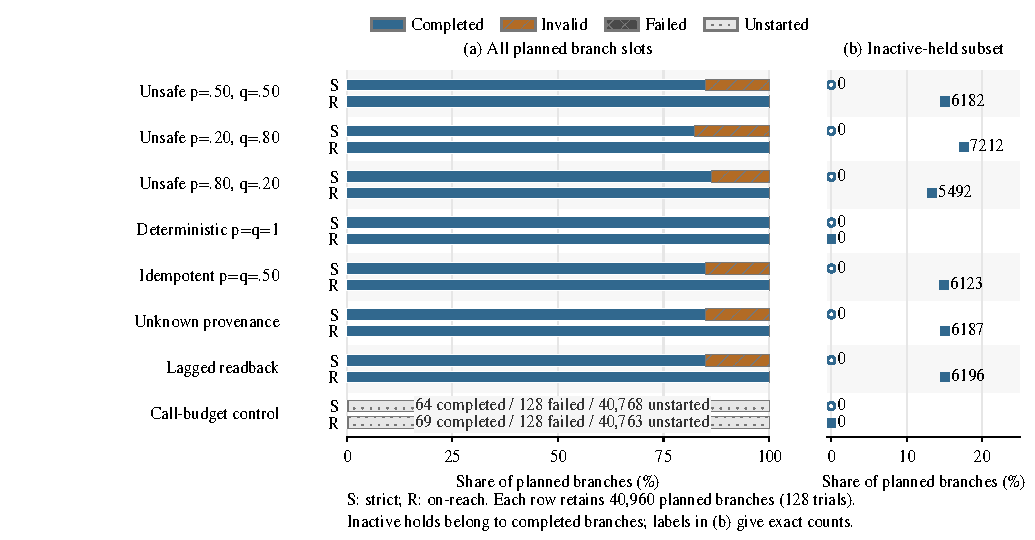
\includegraphics[width=\textwidth]{data-branch-disposition.pdf}
\caption{Disposition of all planned branches across eight mechanisms and two
games: 40,960 slots per row. Completed execution includes unknown target
evidence and known violations; it does not establish an available coefficient.
Failed and unstarted budget-control slots remain visible through exact counts.
Inactive holds are a subset of completed branches, shown separately.}
\label{fig:branches}
\end{figure*}

A standalone auditor importing no framework implementation checked the retained
trials, branches, 4,210 complete traces and all summary rows.
Its receipt binds the frozen source revision and original
52-file manifest. Derived tables retain every row separately from that sealed
collection; auditing made no generation calls.

Actual-call cost also depends on availability. The on-reach unsafe
$(0.5,0.5)$ stratum used 42,526 scripted calls for 128 available global-consequence
coefficient vectors, or 332.23 calls per vector, including factual capture and
independent endpoints. Each vector contains three jointly estimated players.
The lagged stratum spent 42,424 calls for zero such vectors; its cost-per-usable
vector ratio is undefined. Shared targets and interval variants do not multiply
the number of independent usable vectors. These are scripted-call costs, not
production latency or financial charges.

\begin{table*}[t]
\caption{All eight declared cases: on-reach retry coefficient for global
consequence, 128 planned repetitions per row. N/H denotes normal/Hoeffding.
Availability A and population-reference eligibility R each have denominator 128.
Flags denote correct directional detection for nonzero references and false
nonzero flags for zero references. Dashes denote undefined quantities;
0/0 denotes an undefined coverage rate. Hoeffding intervals are clipped to
$[-1,1]$, explaining the 0.773 mean width at $(0.8,0.2)$ versus the
unclipped 0.960 width at the two other stochastic unsafe settings.}
\label{tab:repeated}
\centering\footnotesize
\begin{tabular}{lrrrrr}
\toprule
Case $(p,q)$ or control & Reference & A ; R & Covered N / H & Mean width N / H & Flags N / H\\
\midrule
Unsafe $(0.5,0.5)$ & 0.375 & 128 ; 128 & 118/128 ; 128/128 & 0.226 / 0.960 & 128/128 ; 8/128\\
Unsafe $(0.2,0.8)$ & 0.120 & 128 ; 128 & 124/128 ; 128/128 & 0.154 / 0.960 & 123/128 ; 0/128\\
Unsafe $(0.8,0.2)$ & 0.720 & 128 ; 128 & 123/128 ; 128/128 & 0.218 / 0.773 & 128/128 ; 128/128\\
Deterministic $(1,1)$ & 0 & 128 ; 128 & 128/128 ; 128/128 & 0 / 0.960 & 0/128 ; 0/128\\
Idempotent $(0.5,0.5)$ & 0 & 128 ; 128 & 123/128 ; 128/128 & 0.244 / 0.960 & 5/128 ; 0/128\\
No provenance $(0.5,0.5)$ & 0.375 & 128 ; 128 & 120/128 ; 128/128 & 0.228 / 0.960 & 128/128 ; 7/128\\
Lagged readback $(0.5,0.5)$ & --- & 0 ; 0 & 0/0 ; 0/0 & --- & ---\\
Four-call cap $(0.5,0.5)$ & 0.375 & 0 ; 128 & 0/0 ; 0/0 & --- & ---\\
\bottomrule
\end{tabular}
\end{table*}

\begin{figure*}[t]
\centering
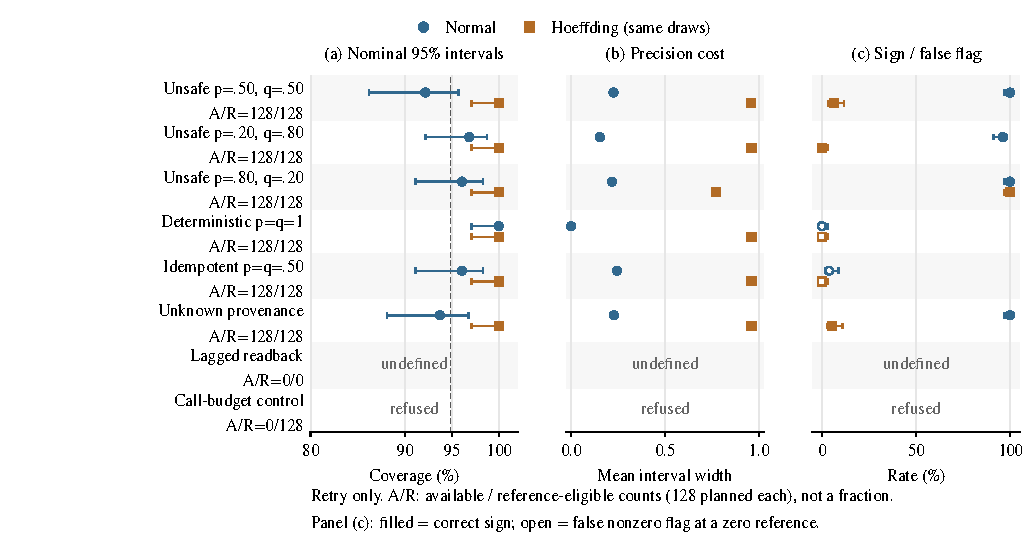
\includegraphics[width=\textwidth]{data-interval-tradeoffs.pdf}
\caption{On-reach global-consequence retry coefficient for all eight cases,
using identical draws for both interval methods. A/R denotes available and
population-reference-eligible counts, each from 128 planned trials. Coverage
and flag whiskers are 95\% Wilson uncertainty for repeated-trial rates, not
coefficient intervals. Filled flag markers indicate correct directional
detection; open markers indicate false nonzero flags for zero-reference
controls. Undefined evidence and budget refusals have no zero-valued markers.}
\label{fig:tradeoffs}
\end{figure*}

Table~\ref{tab:repeated} reports every declared mechanism for one specified
target and position, including unavailable controls.
Figure~\ref{fig:tradeoffs} places coverage beside interval width and detection
to expose their tradeoff without pooling targets or cases. At $(p,q)=(0.5,0.5)$,
the shared retry estimate had bias $-0.00269$ and RMSE 0.0611. Normal coverage
118/128 has a 95\% Wilson interval $[0.862,0.957]$; 128/128 has
$[0.971,1]$, not proof of perfect population coverage. The conservative
intervals sharply reduced weak-effect sign detection. For the consequence
stop dummy, normal false nonzero flags ranged from 0 to 14/128 across the six
assessable mechanisms; Hoeffding flags were 0/128 in each. The deterministic
zero-reference case yielded 128 normal point intervals; their correctness in
that case does not validate point intervals for stochastic outcomes.
With 128 repetitions, $[0.862,0.957]$ also shows why an observed 92.2\% rate
does not resolve a small departure from 95\% coverage. These runs are diagnostic
integration evidence, not a precise empirical ranking of near-nominal methods.
The finite-distribution calculation supplies a separate analytic check only
for its declared independent Bernoulli law.

Endpoint behavior was separately assessed. For the on-reach unsafe
$(0.2,0.8)$ global-consequence endpoint,
normal coverage was 92/128 (Wilson $[0.635,0.789]$), with 35 point intervals
and mean width 0.114. Exact-marginal differences covered 128/128, with mean
width 0.319. These finite results demonstrate the declared precision tradeoff;
they do not establish simultaneous coverage or calibration under live-model
dependence.

In the on-reach game, every lagged-consequence coefficient was refused as
unknown; every budget
coefficient was refused after unstarted slots, despite the latter's defined
ideal reference. Removing provenance preserved global-consequence availability
but refused all 128 linked-consequence coefficient vectors. All nondeterministic strict
coefficient vectors were unavailable and their population games undefined;
the fully deterministic strict control remained defined. One finite strict
interaction point at $(0.8,0.2)$ did not make that population interaction
defined. One strict linked-consequence endpoint without provenance was numeric
but reference-ineligible, giving coverage 0/0 rather than an accuracy result.
Pooled-coalition interaction diagnostics have no confidence interval
and supply no coverage or sign-detection result. The full summary retains
separate availability, reference eligibility, bias/RMSE, coverage uncertainty,
width, flags, endpoints, interactions and refusal rows for every target,
position, game and interval variant. Reused targets and variants are not
independent replications.

\subsection{Exploratory local-model validation}
A frozen installed Qwen3 4B checkpoint completed six validation cases,
two repetitions and two unchanged prompt profiles, using 59 actual calls
within a 72-call cap. No episode failed or remained unstarted. Model identity,
prompt/payload hashes, public traces and the exact source checkpoint are retained.
The original and revised profiles induced different action sequences; this
is not a pure reporting experiment or an attribution-method comparison.

\begin{table}[t]
\caption{Local-model validation with explicit claim denominators.}
\label{tab:model}
\centering\footnotesize
\begin{tabular}{lrr}
\toprule
Quantity & Original v1 & Revised v2\\
\midrule
Completed/planned episodes & 12/12 & 12/12\\
Actual calls/profile cap & 36/36 & 23/36\\
Definite final status claims & 12/12 & 0/12\\
Contradictions/assessable claims & 6/10 & 0/0\\
State satisfied/violated/unknown & 6/4/2 & 7/3/2\\
Linked satisfied/false/unknown & 6/4/2 & 5/5/2\\
\bottomrule
\end{tabular}
\end{table}

The revised profile's conditional contradiction rate is undefined, not zero
error. The original profile's 6/10 contradiction proportion has a descriptive
95\% Wilson interval of approximately $[0.313,0.832]$. Shared cases, fixed
profile order and two repetitions per case preclude interpreting this interval
as calibrated uncertainty over a broader population of tasks or models.
In the other-actor case, revised-profile readback satisfied state while
origin was external and action linkage false. In the expired-request case,
the original profile correctly described ineligibility but issued a refund;
its failure assessment contradicted achieved effect. Effect satisfaction and
eligibility-policy correctness are distinct targets.

A separate unblinded annotation pass within the AI-assisted development
workflow marked affirmative processing clauses in 10/12 original and 7/12
revised final rationales. Five of those
seven revised rationales also hedged independent verification. A statement
that a second attempt committed can be literally true while two effects
violate an exactly-one task. These annotations are descriptive; no independent
human verification or inter-rater reliability has been established. Unknown
structured fields do not ensure prose abstention. The saved auditor rejected
seven corrupted smoke copies without additional generation. Fixed profile order,
tiny sample size, shared fault conditions and an exposed validation family
limit interpretation. The held-out reserve was not generated.

\section{Discussion and Limitations}
The evidence protocol supports different, inspectable claims about responses,
state, origin and intervention effects. Its refusal rules prevent unsupported
numerical outputs but can sharply reduce availability. Availability can depend
on interventions and must remain visible beside numerical results. Conservative
intervals do not make undefined games numeric, resolve missing evidence, or
remove the need to assess the actual sampling law.

The environment is a narrow scripted simulator. No real payment API or standard
world-state benchmark was evaluated. The artifact-delivery example validates
an integration interface, not a second production-domain experiment. Declared
source authority and watermarks are not authenticated transactional guarantees.
The model experiments use one local model and exposed development/validation
families; they do not estimate broad model performance or held-out transfer.
State and linked targets sharing outcomes are not independent replications.
Claims about hidden reasoning cannot be inferred from reported assessments.

Three evaluation gaps determine the next study design. First, compare a
response-only auditor, a verify-before-retry wrapper, a faithful CAR-style
adapter, an LLM trace judge and simple last-step rules on identical fault
traces. State satisfaction, source-supported origin and causal intervention
effects need separate reference labels. Report duplicate effects, false success
claims, abstention/availability, attribution accuracy and actual cost under
matched evidence, targets and call budgets. Joint context/fault attribution
must expose infrastructure variables to every applicable method.

Second, assess bounded polling on an eventually consistent readback: poll
until its declared watermark covers the horizon or a predeclared wait budget
expires, then retain unknown. Report availability against wait time, read
count and latency. Polling cannot promise finality or exactly-once execution
under arbitrary late commits. The retained lag control uses one insufficient
readback and yields zero consequence estimates; a polling result has not been
measured. A safe real-service study would use provider test mode, isolated
accounts and injected acknowledgement faults; counterfactual replay would
remain in an isolated simulator or a separately validated digital twin.

Third, preregister held-out template and fault-composition families, multiple
model classes and independent blinded double annotation with agreement
reporting. A planned 3--5-model, 500-or-more-episode study requires a precision
and clustering analysis before fixing its final sample size. At least 1,000
independent repetitions per selected simulator setting would better resolve
coverage, with simultaneous uncertainty over predeclared positions and
modern bounded-mean interval comparators. These are proposed experiments.
No matched baseline, polling study, multi-model result or human annotation
agreement is claimed here.

The retained cost record counts actual scripted calls and refusals; the repeated
study used 628,535 calls and zero model calls. It does not measure per-call
verification latency, trace-size overhead, real-API charges or cost per usable
production estimate. Those measurements belong in the next evaluation.

\section{Conclusion and Artifact Availability}
Consequa-X provides a reusable evidence core and auditable replay adapters for
separating reported assessments, external outcomes, origin and intervention
effects. The retained studies expose uncertainty failure, precision costs,
variable-length game restrictions and prose/structured-status disagreement.
The useful result is a reproducible protocol/software artifact with measured
limits, without claiming a new estimator or general method superiority.

Stable version 1.1.0 is publicly available under MIT on PyPI~\cite{artifact}.
Its wheel and source distribution were independently downloaded and
hash-checked, and an isolated registry installation was verified on
October 17, 2026. The wheel contains the
runtime, schemas and typing marker; the source distribution also includes
documentation, offline examples, tests and audit scripts. Private research
outputs and model weights are excluded. The maintainer-controlled repository
at \url{https://github.com/Devrajsinh-Jhala/consequa-x} is private. Git history,
retained protocols, raw evidence and evaluator-only truth are retained there
for authorized collaborators; this paper does not assert unrestricted access
to that research archive.
The experiments predate the 1.1.0 release: original calibration used source
\texttt{9e2dcbb}, shared-draw comparison \texttt{0d8ec0b}, refund enumeration
and local validation \texttt{2c4adfe}, and repeated sampling \texttt{0bd744d}.
Full revisions and manifests are retained in the evidence ledger. Version
1.1.0 adds current engineering interfaces and offline reports; its publication
does not rerun or change those historical studies. A public immutable
research archive and review-access arrangements have not been established.
Framework imports and offline examples require no model credentials or required
runtime dependencies. All reported payments are simulated; model weights are
identified rather than redistributed.

\section*{AI Assistance and Verification Disclosure}
Generative AI assistance was used for software development, research-source
inspection, rationale annotation and manuscript drafting. Recorded automated
checks cover retained-evidence accounting, analytic references, numerical
implementations and document compilation. They do not constitute independent
human replication or blinded annotation. The rationale labels remain unblinded
and exploratory. The author is responsible for the paper's claims and any
venue-required disclosure; no independent human validation is asserted.

\appendices
\section{Declared-Game Properties and Test Evidence}
\label{app:games}
\textbf{Strict-game partiality.} In the declared three-position mechanism,
let $N=\{s,r,t\}$ be selection, timeout retry and final stop. If $p<1$, the
coalition $\{r\}$ requests a retry that is unreachable with probability
$1-p>0$ when fresh selection declines. If $q<1$, coalition
$\{s,t\}$ holds selection and requests a final stop that is unreachable with
probability $1-q>0$ when the fresh timeout decision stops. With compatible
decisions, normal execution, adequate budget and known outcomes, the full strict
coalition game is structurally defined if and only if $p=q=1$ in this mechanism.
In particular the full strict game is partial at every interior $(p,q)$ and
ordinary full-game Shapley is undefined there. Conditioning on valid replay
would define a different game. A finite sample with no invalid draw cannot
establish zero population invalid probability.

\textbf{On-reach allocation.} Fix finite factual positions, an intervention
mapping and a continuation law. Suppose each coalition terminates almost surely,
all reached held decisions are compatible, and a bounded measurable numeric
outcome exists almost surely. Ignoring holds beyond normal termination then
defines $v(S)=\mathbb{E}[X_S]$ for every coalition. Its ordinary Shapley values
obey efficiency, symmetry, the null-player property and linearity. To see
efficiency, sum the marginal contributions along each permutation: they
telescope to $v(N)-v(\varnothing)$, and averaging preserves the equality.
Relabelling permutations gives symmetry; zero marginals give the null-player
property; linearity follows from linearity of each difference and of averaging.
These properties belong to this declared game. They establish neither causal
identifiability nor nonnegative normalized responsibility. Unknown observations,
incompatible holds and provider failures remain outside these assumptions.
Finite independently sampled coalition values can give a nonzero estimate for
a true null player, and an independently sampled endpoint need not equal the
sum of finite estimated shares.
Uniform forward permutations and their reverses each have a uniform marginal.
With unbiased coalition samples, their paired average is unbiased for the
declared Shapley value. Independent pairs, rather than individual walk steps,
are the sampling units for the bounded-mean interval.

\textbf{Test mapping.} C1 is exercised by external-actor and absent-provenance
tests in \texttt{test\_verification.py} and conflicting-observation tests in
\texttt{test\_graph\_identity.py}. C2 is exercised by
\texttt{test\_refund\_interactions.py}, the exact-rational analytic checker,
and retained enumeration controls. C3 is exercised by unknown-draw and
exhausted-budget tests in \texttt{test\_decision\_shapley.py}, plus the
saved-evidence branch audit. Tests establish behavior in their stated cases,
not correctness of an untrusted source or a real-service policy.

\section{Supporting Audit Inventory}
Raw assertion counts are retained for reproducibility rather than treated as
evidence strength: 3,283,523 for the shared-draw audit, 27,277 for the enumeration
audit, 44,698,925 for repeated sampling, and 2,227 for the local validation.
These counts depend on data volume and auditor implementation. More informative
checks include independently recomputed summaries, exact-rational analytic
references, source-bound inventories, refusal denominators and rejected
semantic corruptions. None supplies independent human verification.

\IEEEtriggeratref{9}
\begin{thebibliography}{99}
\bibitem{car} J. Shah, ``Causal Agent Replay: Counterfactual Attribution for
LLM-Agent Failures,'' arXiv:2606.08275, v1, Jun. 2026.
\bibitem{pccc} R. Meng, ``Policy-Conditioned Counterfactual Credit for Verifiable
Reinforcement Learning of Long-Horizon Language Agents,'' arXiv:2606.05263, v1,
Jun. 2026.
\bibitem{causalloss} A. Sharma, ``CausalLoss-Fin: Attributing Financial-Agent
Loss to Decisions and Infrastructure Faults,'' arXiv:2609.25960, v1, Sep. 2026.
\bibitem{verified} I. K. Mansoor, A. Phadke, and P. Rana, ``Verified Tool Calls
Improve LLM Agent Reliability Under Non-Atomic Failures,'' arXiv:2608.02645,
v1, Jul. 2026.
\bibitem{operability} Z. Wang, ``Callability Is Not Operability: Controlled
Interface Interventions for LLM Agents,'' arXiv:2608.23628, v2, Aug. 2026.
\bibitem{whoandwhen}
S. Zhang \emph{et al.}, ``Which Agent Causes Task Failures and When? On Automated Failure Attribution of LLM Multi-Agent Systems,'' in \emph{Proc. 42nd Int. Conf. Machine Learning}, PMLR, vol. 267, 2025, pp. 76583--76599. [Online]. Available: \url{https://proceedings.mlr.press/v267/zhang25cq.html}
\bibitem{prov}
L. Moreau and P. Missier, Eds., ``PROV-DM: The PROV Data Model,'' W3C Recommendation, Apr. 30, 2013. [Online]. Available: \url{https://www.w3.org/TR/2013/REC-prov-dm-20130430/}
\bibitem{agenttool}
A. Trofimov and B. Novikov, ``When Tool Calls Succeed but Workflows Fail: Anomalies at the Agent-Tool Boundary,'' arXiv:2609.15397v1, 2026. [Online]. Available: \url{https://arxiv.org/html/2609.15397v1}
\bibitem{limbo}
J. Li, ``Where Does Exactly-Once Live? Model, Harness, and Tool-Contract Effects on Duplicate Side Effects in LLM Agents,'' arXiv:2609.29095v1, 2026. [Online]. Available: \url{https://arxiv.org/html/2609.29095v1}
\bibitem{helland}
P. Helland, ``Idempotence Is Not a Medical Condition,'' \emph{Communications of the ACM}, vol. 55, no. 5, pp. 56--65, 2012, doi: 10.1145/2160718.2160734.
\bibitem{vogels}
W. Vogels, ``Eventually Consistent,'' \emph{Communications of the ACM}, vol. 52, no. 1, pp. 40--44, 2009, doi: 10.1145/1435417.1435432.
\bibitem{appworld}
H. Trivedi \emph{et al.}, ``AppWorld: A Controllable World of Apps and People for Benchmarking Interactive Coding Agents,'' in \emph{Proc. 62nd Annu. Meeting Association for Computational Linguistics}, vol. 1, 2024, pp. 16022--16076, doi: 10.18653/v1/2024.acl-long.850.
\bibitem{toolsandbox}
J. Lu \emph{et al.}, ``ToolSandbox: A Stateful, Conversational, Interactive Evaluation Benchmark for LLM Tool Use Capabilities,'' in \emph{Findings of the Association for Computational Linguistics: NAACL 2025}, 2025, pp. 1160--1183, doi: 10.18653/v1/2025.findings-naacl.65.
\bibitem{taubench}
S. Yao, N. Shinn, P. Razavi, and K. Narasimhan, ``$\tau$-bench: A Benchmark for Tool-Agent-User Interaction in Real-World Domains,'' arXiv:2406.12045v1, 2024. [Online]. Available: \url{https://arxiv.org/html/2406.12045v1}
\bibitem{brown}
L. D. Brown, T. T. Cai, and A. DasGupta, ``Interval Estimation for a Binomial Proportion,'' \emph{Statistical Science}, vol. 16, no. 2, pp. 101--133, 2001, doi: 10.1214/ss/1009213286.
\bibitem{betting}
I. Waudby-Smith and A. Ramdas, ``Estimating Means of Bounded Random Variables by Betting,'' \emph{Journal of the Royal Statistical Society Series B: Statistical Methodology}, vol. 86, no. 1, pp. 1--27, 2024, doi: 10.1093/jrsssb/qkad009.
\bibitem{shapley} L. S. Shapley, ``A Value for N-Person Games,'' RAND
Corporation, P-295, 1952, doi: 10.7249/P0295.
\bibitem{clopperpearson}
C. J. Clopper and E. S. Pearson, ``The Use of Confidence or Fiducial Limits Illustrated in the Case of the Binomial,'' \emph{Biometrika}, vol. 26, no. 4, pp. 404--413, 1934, doi: 10.1093/biomet/26.4.404.
\bibitem{hoeffding} W. Hoeffding, ``Probability Inequalities for Sums of
Bounded Random Variables,'' Journal of the American Statistical Association,
vol. 58, no. 301, pp. 13--30, 1963.
\bibitem{artifact} D. Jhala, ``Consequa-X,'' MIT Python distribution,
ver. 1.1.0, Oct. 17, 2026. [Online]. Available:
\url{https://pypi.org/project/consequa-x/1.1.0/}
\end{thebibliography}
\end{document}
